% dibuix_esfera_2.tex
\documentclass{standalone}
\usepackage{tikz}
\usetikzlibrary{arrows.meta, decorations.markings}

\begin{document}

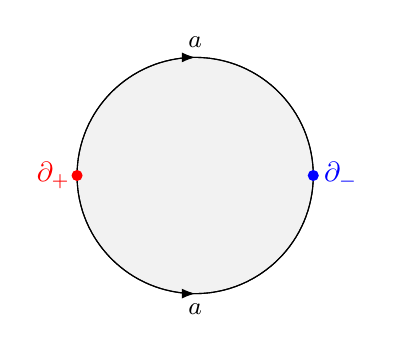
\begin{tikzpicture}[
    identified_edge/.style={
        decoration={
            markings,
            mark=at position 0.5 with {\arrow{Latex}}
        },
        postaction={decorate}
    },
    edge_label/.style={midway, auto, font=\small}
]

\def\circle_size{1.5}

% Draw circle
\draw[fill=gray!10] (0,0) circle (\circle_size);

% Draw identified semicircles
\draw[identified_edge] (-\circle_size,0) arc(180:0:\circle_size) node[edge_label, above] {$a$};
\draw[identified_edge] (-\circle_size,0) arc(-180:0:\circle_size) node[edge_label, below] {$a$};

\node[red] at (-\circle_size-0.3,0) {$\partial_+$};
\node[blue] at (\circle_size+0.35,0) {$\partial_-$};

% Add dots at the partials
\fill[red] (-\circle_size,0) circle (2pt);
\fill[blue] (\circle_size,0) circle (2pt);

\end{tikzpicture}

\end{document}